\begin{figure*} \centering
  \begin{tabular}{ccc}
    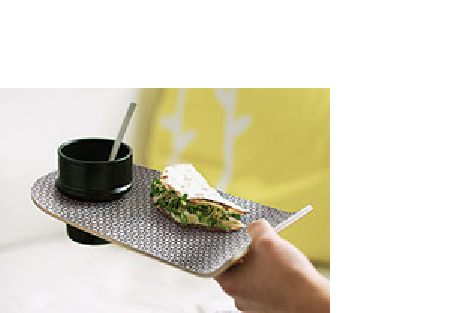
\includegraphics[width=0.25\textwidth]{images/pickup_press.pdf} &
    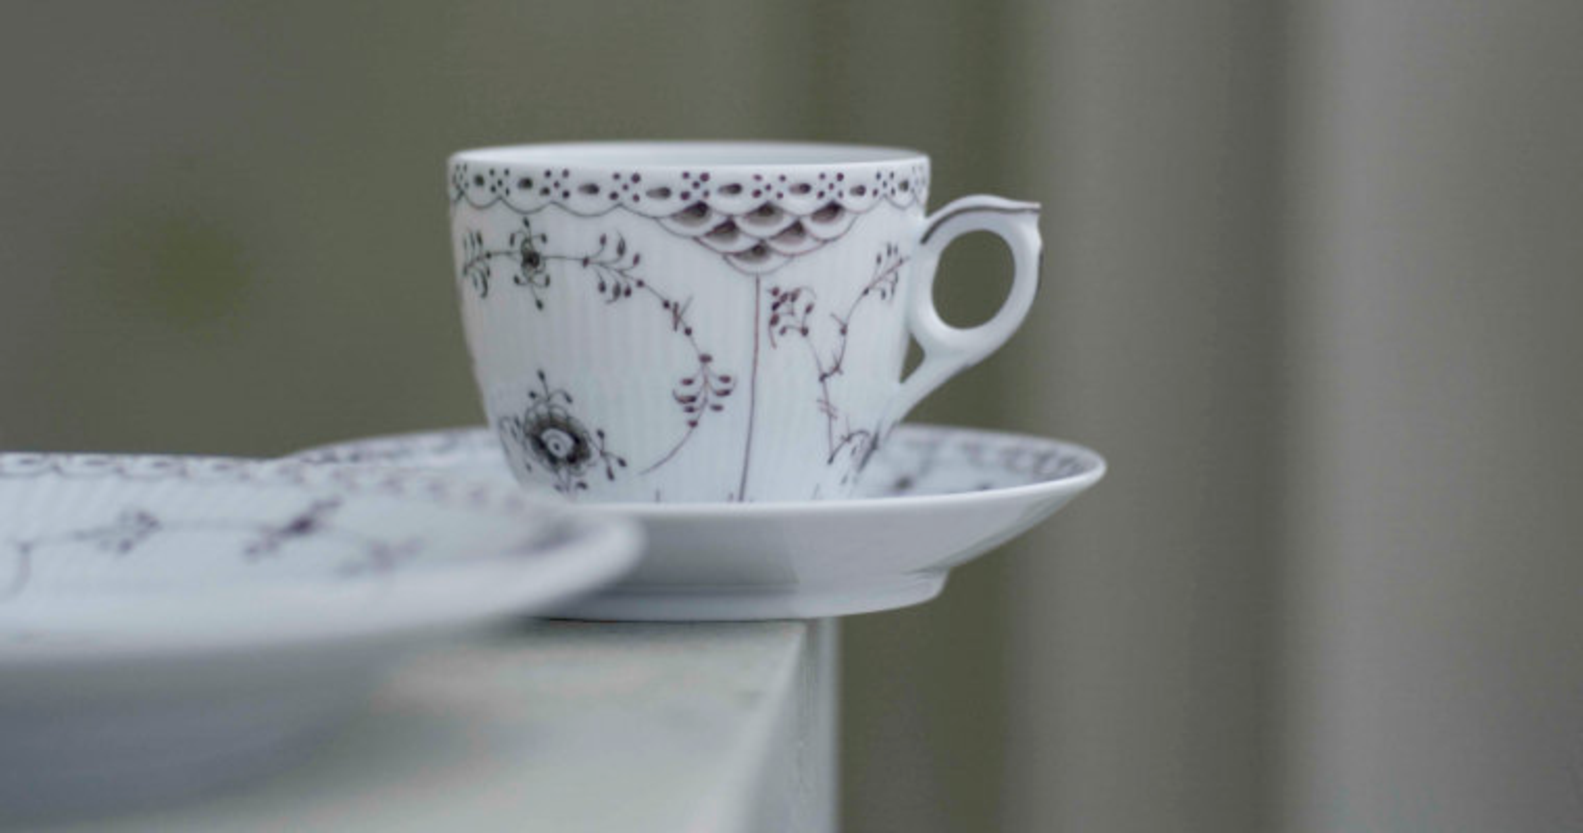
\includegraphics[width=0.25\textwidth]{images/black-fluted-half-lace-2.pdf} &
    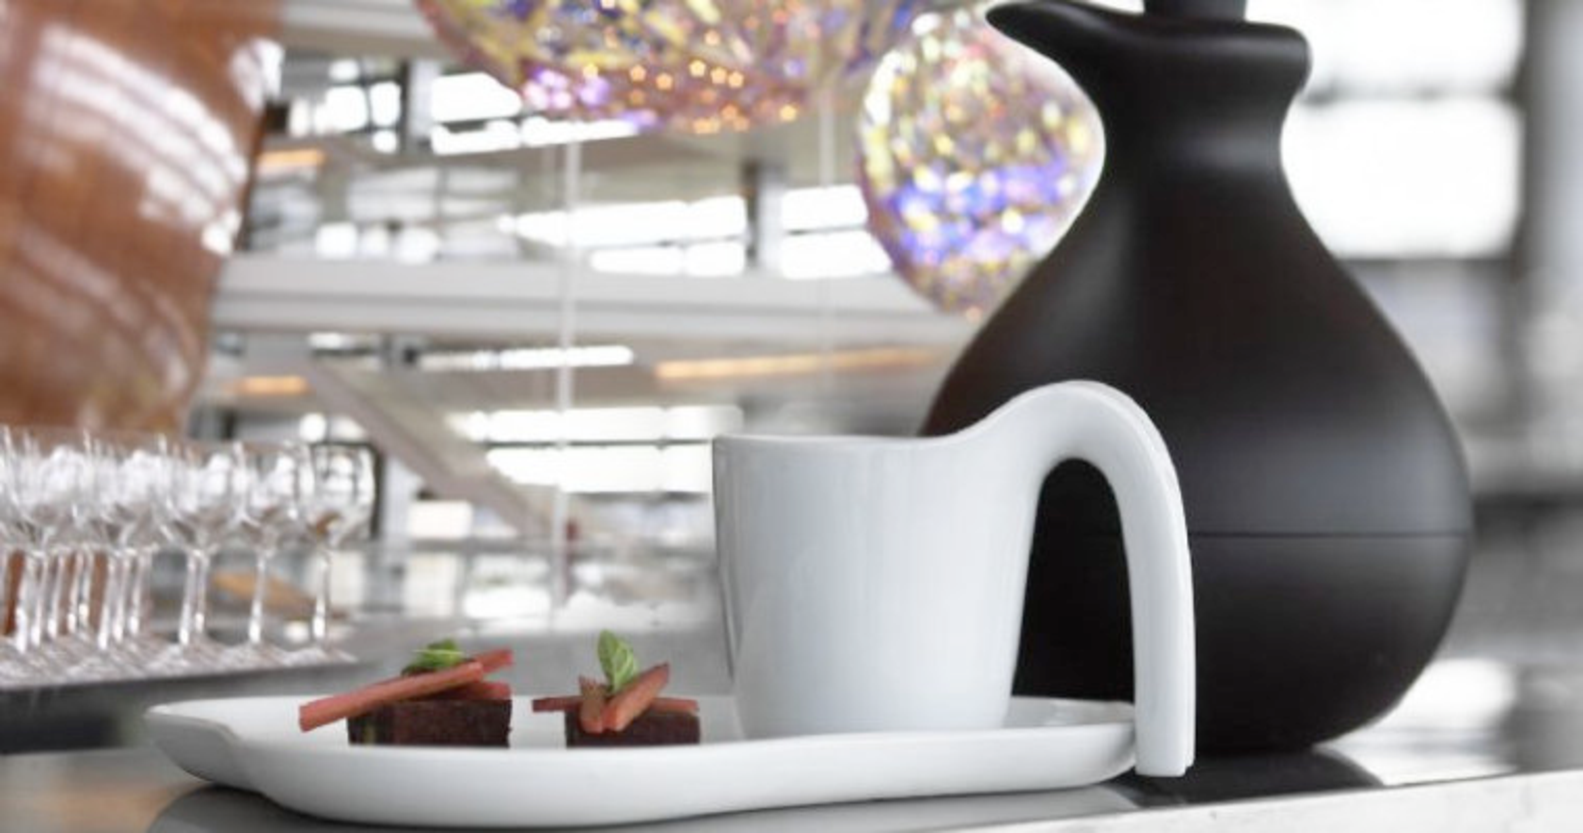
\includegraphics[width=0.25\textwidth]{images/ole-at-opera-3.pdf} \\
  \end{tabular}
  \caption{Three very different cups: (left) the Pick Up mug by H\"ogan\"as (2009);
          (center) the Black Flute Half Lace coffee cup (1775) and (right) the
          'Ole mug (1997), both by Royal Copenhagen.}
  \label{fig:chairs}
\end{figure*}

Consider the objects in Figure \ref{fig:chairs}. How do we know that they are all
cups? The answer is simple: all of them can be used to contain liquids and drink,
and have actually been designed to this end. Although very little in
their visual appearance ties them together, we all know what can be done with such
objects since \emph{we have done it} at some time in the past. The category of an object
is often determined predominantly by its function rather than by its visual appearance
alone; this led Gibson in the 70s \cite{gibson1,gibson2} to define objects
in terms of their affordances --- ``what can be done with them''.

This idea could be useful to improve the classic solution to object recognition,
which uses visual features only. It is hard to figure out
what visual features could lead an object recognition system to categorise as
``cups'' the three objects above. Traditionally, this problem is solved by training
the system on a very large database of images of very diverse cups; but this is
potentially incomplete and resource-consuming \cite{leibe_etal_ijcv2008}.
Now, what if our machines had an idea
of how to \emph{grasp} something which looks like a mug? In fact, if this paradigm is
correct, this could be the reason behind the robustness of human object
recognition. Such robustness could be obtained by automated systems if only
they knew what to do with an object, as they see it. This implies that an
object recognition system must be able to grasp objects, or it must know something
about grasping. Once it does, it has a wholly new way to associate a category
to an object it sees.

In order to test this hypothesis, we have first collected a number of
human grasping sequences, recording at the same time a video sequence of the grasping act
and the hand posture (using a sensorised glove). These sequences are collected in
the CONTACT Visuo-Motor Grasping dataBase (VMGdB)\footnote{Upon acceptance
of the paper, the database will be made available online.}. 

Then, using the VMGdB, by means of a simple
neural network we have built a map from the image of each object to the associated
grasp(s) or, in other words, a Visuo-Motor Map (VMM) from visual to motor features.
The VMM enables us to retrieve the ``archetypal grasp'' of an object when that
object is seen.
The VMM is then used to build a Visuo-Motor Classifier (VMC)
which exploits the traditional visual information plus the associated motor information,
either the ``real'' one, as it was recorded by the glove, or the VMM-reconstructed
one. The latter scenario is of course more realistic, as in most real-life applications,
and in real life as well, the only available input is visual.
%During training, we learn how to
%exploit optimally the informative content of the two sensory channels so to achieve
%the best possible performance --- this is obtained by determining the optimal
%similarity measure for each modality, and how much to weight each of them when
%combining the channels together. \textbf{cc: poco chiara questa frase}
%During testing, when visual features only are available, the VMM generates the
%corresponding sensorimotor features (an archetipal grasp associated to an object),
%enabling to use both modalities for classification. Hopefully, this enhanced
%classification is better than that done with visual features alone.
The hope is that this augmented object classifier performs dramatically better
than the standard one when the real motor features are added; and significantly
better when the reconstructed ones are used. Our experimental results clearly
confirm this hypothesis.

The paper is organised like this: after an overview of related work, in Section
\ref{sec:database} we describe the Visuo-Motor Grasping dataBase (VMGdB).
Section \ref{sec::framework}  defines the general multi-modal learning framework, and
then it describes in detail the instance under examination:
the visual and motor representation (\ref{sec::vision}),
the Visuo-Motor Map (VMM, Section \ref{sec::regression}) and 
the Visuo-Motor Classifier  (VMC, Section \ref{sec::classifier}). 
We then show the
experimental results (Section \ref{sec::experiments}) and draw  conclusions
in Section \ref{sec::conclu}.

% quel che segue secondo me non fa piu` filare il discorso...
%
%Inspired by these considerations, we hereby define a theoretical framework for
%reconstructing \emph{active} sensory modalities, i.e., those by which we explore
%the world, from \emph{passive} ones, i.e., those by which we receive information
%about it. We focus on manipulable objects and build a mapping between the visual
%appearance of an object and the sensorimotor information about it, corresponding
%to a grasp associated to the object. \textbf{babi: non sono certo di volere
%mantenere in piedi il discoro del ``theoretical framework for...'' Forse sarebbe
%meglio andare diretti al punto della ricostruzione visuomotoria.}

%, that is in
%short, for figuring out what to do with what one sees, hears, smells etc. In particular,
%we enforce one such schema using a multi-variate regression technique to associate
%\emph{object visual features} to related \emph{human grasping postures}. This schema is
%called a \emph{Visuo-Motor Map} (VMM) and is trained
%using a large database of visual and motor data collected from human subjects, that
%we call the \emph{Visuo-Motor Grasping dataBase} (VMGdB). The immediate result is the
%ability of retrieving a (set of) grasping posture(s) just by seeing an object; this
%ability, which we call \emph{grasp priming}, has obvious applications in robotic fields
%where (semi)autonomous grasping / fine manipulation is reuquired, such as robotic surgery,
%humanoid robotics, teleoperation, advanced hand prosthetics etc. This connection between
%robotics and the mirror theory has been explored, although not to this extent, at
%least in \cite{lopes-05,metta-06}.
%
%Notice that this problem is, in general, ill-posed, since an object can be grasped in
%many distinct ways: a direct inverse mapping from visual to motor features is impossible.
%So we resort to a probabilistic estimation: given the sight of an object, how would I
%\emph{most likely} grasp it? This solution is similar to that found for motor-based speech
%recognition, e.g., in \cite{richmond2007}. More in detail, \textbf{ANNALISA e DISI-jin, volete
%approfondire brevemente?}
%
%Lastly, since the focus of this work is on enhancing object reocgnition, we show
%that the grasping posture estimation reconstructed by the VMM dramatically improves the
%classification rate of a standard object classifier. The visual/motor cue integration is
%realised via \textbf{BABI, TATIANA, questo e` vostro}. Our experimental analysis shows
%that \textbf{e qui mettiamo i numeri principali dei risultati sperimantali.}

%\begin{itemize}
%
%\item learning by imitation great capability of cognitive systems. It permits to learn how to grasp a cup never seen before just by seeing someone else doing it.
%Fundamental learning mechanism etc 
%
%\item a widely accredited hip is that the underlying mechanism of learning by imitation is the existence of a sensor motor map that links
%the visual perception of an object to the motir position of the hand when it manipulates it. Mirror neurons blabla 
%
%\item another consequence of the existence of a sensor-motor map is that when we learn an object by seeing and manipulating it, we are then able
%to recognize it with a higher degree of accuracy and robustness than if we would have learned it on visual data only. 
%
%\item Enabling a robot to display similar abilities is one of the holy grails of research in artificial cognitive systems. 
%
%\item In this paper we present a mirror neurons inspired algorithm for building perception action maps between visual, passive perception and motor, active
%perception. During learning, the algorithm takes as input visual and sensomotor data and (a) it builds a mapping between the two modalities (b) it builds 
%a classifier on both modalities. After training, wehn presented with a visual input, the system is able to perform grasp priming (= is able to predict
%which are the possible way to grasp the seen object; this information could be used to pre-activate a robot hand) and enhanced visual recognition
%(= is able to recognize objects with a higher degree of accuracy and robustness compared to a model learned only on visual features, even if
%the sensor modality is not perceived by the agent). Experiments show that.....
%
%\item in the rest of the paper...
%
%\end{itemize}
